\chapter{Parallel Computing}
Parallel computing is a form of computation in which many instructions are carried out simultaneously (see \autoref{fig:screenshot051}). It operates on the principle that large problems can often be divided into smaller ones, which are then solved concurrently. There are several different forms of parallel computing: bit-level parallelism, instruction-level parallelism, data parallelism, and task parallelism. 
\begin{figure}
\centering
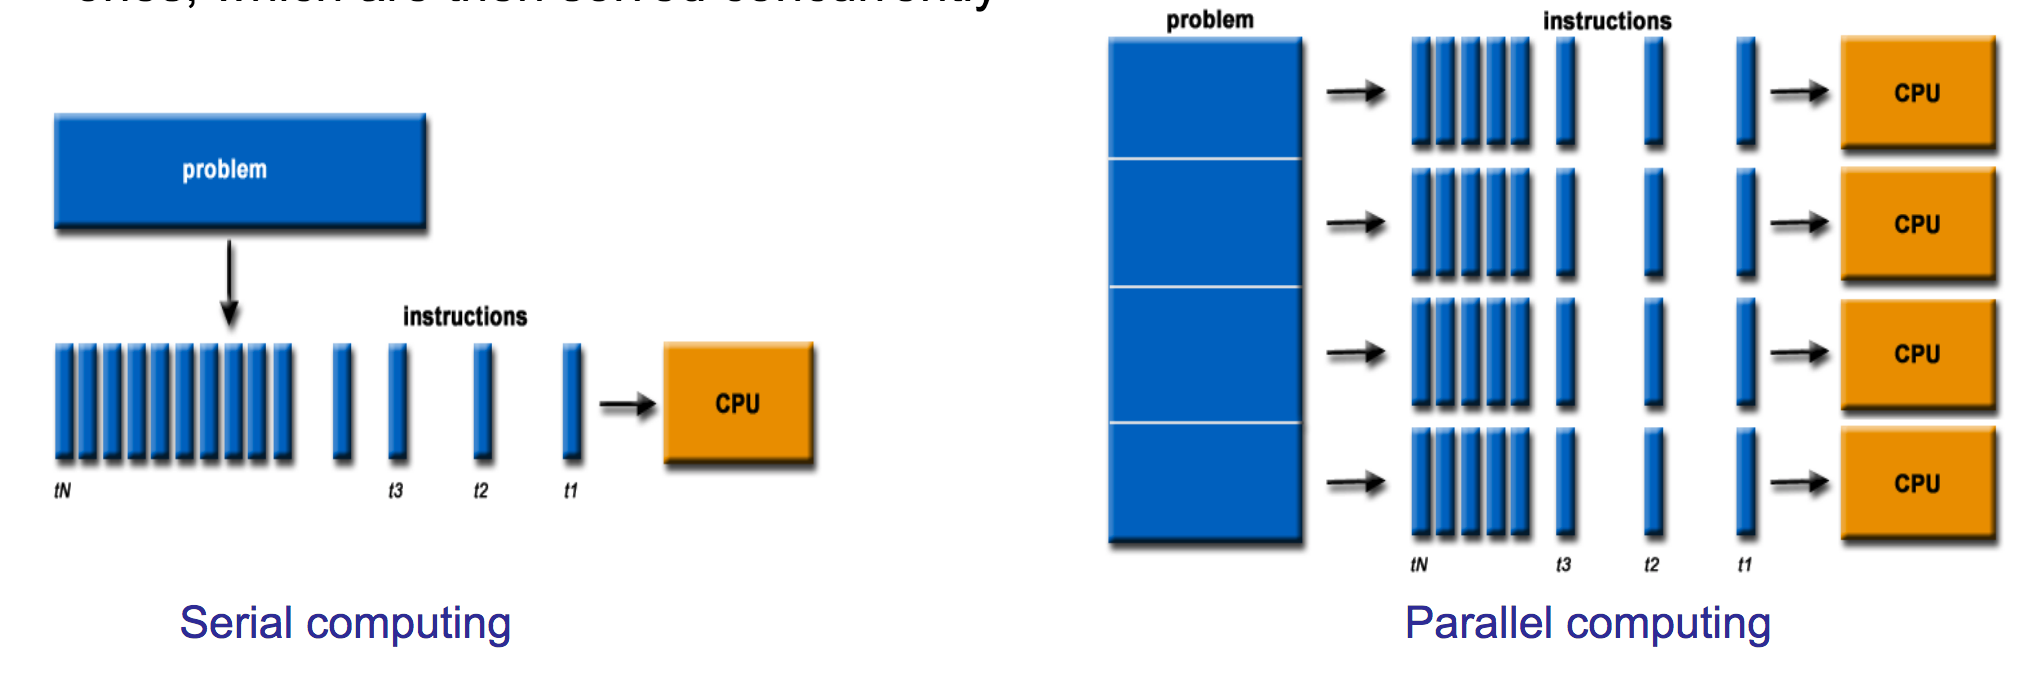
\includegraphics[width=0.7\linewidth]{figures/screenshot051}
\caption{Serial computing vs parallel computing.}
\label{fig:screenshot051}
\end{figure}

Contemporary computer applications require the processing of large amounts of data in sophisticated ways. Examples include:  \begin{itemize}
\item parallel databases, data mining  
\item oil exploration  
\item web search engines, web based business services  
\item computer-aided diagnosis in medicine  
\item management of national and multi-national corporations  
\item advanced graphics and virtual reality, particularly in the entertainment industry  
\item networked video and multi-media technologies  
\item collaborative work environments  
\end{itemize}
Ultimately, parallel computing is an attempt to minimise computational time and effort. 

There are different ways to classify parallel computers. One of the more widely used classifications, in use since 1966, is Flynn's taxonomy.  Flynn's taxonomy distinguishes multi-processor computer architectures according to two independent dimensions of Instruction and Data. Each of these dimensions can have only one of two possible states: Single or Multiple.  This lends itself to the four possible classifications, shown in \autoref{fig:screenshot052}:
\begin{itemize}
\item \textbf{Single Instruction, Single Data (SISD)}: A serial (non-parallel) computer; executes deterministically. This is the oldest and until recently, the most prevalent form of computer. Examples: most PCs, single CPU workstations and mainframes.

\textit{Single instruction}: Only one instruction stream is being acted on by the CPU during any one clock cycle. 

\textit{Single data}: Only one data stream is being used as input during any one clock cycle. 

\item \textbf{Single Instruction, Multiple Data (SIMD)}: A type of parallel computer best suited for specialized problems characterized by a high degree of regularity, such as image processing; it features synchronous (lockstep) and deterministic execution. This type of machine typically has an instruction dispatcher, a very high-bandwidth internal network, and a very large array of very small-capacity instruction units.

Two varieties: Processor Arrays and Vector Pipelines. Examples for processor arrays: Connection Machine CM-2, Maspar MP-1, MP-2. Examples for vector pipelines: IBM 9000, Cray C90, Fujitsu VP, NEC SX-2, Hitachi S820.

\textit{Single instruction}: All processing units execute the same instruction at any given clock cycle.

\textit{Multiple data}: Each processing unit can operate on a different data element.

\item \textbf{Multiple Instruction, Single Data (MISD)}: A single data stream is fed into multiple processing units. Each processing unit operates on data independently via independent instruction streams. 

\textit{Multiple instruction}: Every processor may be executing a different instruction stream.

\textit{Single data}: Only one data stream is being used as input during any one clock cycle. 

Few actual examples of this class of parallel computer have ever existed. One is the experimental Carnegie-Mellon computer. Some conceivable uses might be:  \begin{itemize}
\item multiple frequency filters operating on a single signal stream  
\item multiple cryptography algorithms attempting to crack a single coded message.  
\end{itemize}

\item \textbf{Multiple Instruction, Multiple Data (MIMD)}: Currently, the most common type of parallel computer. Most modern computers fall 
into this category. Execution can be synchronous or asynchronous, and deterministic or non-deterministic. Examples: most current supercomputers, networked parallel computer "grids" and multi-processor SMP computers - including some types of PCs.  

\textit{Multiple instruction}: Every processor may be executing a different instruction stream.

\textit{Multiple data}: Each processing unit can operate on a different data element.
\end{itemize}

\begin{figure}
\centering
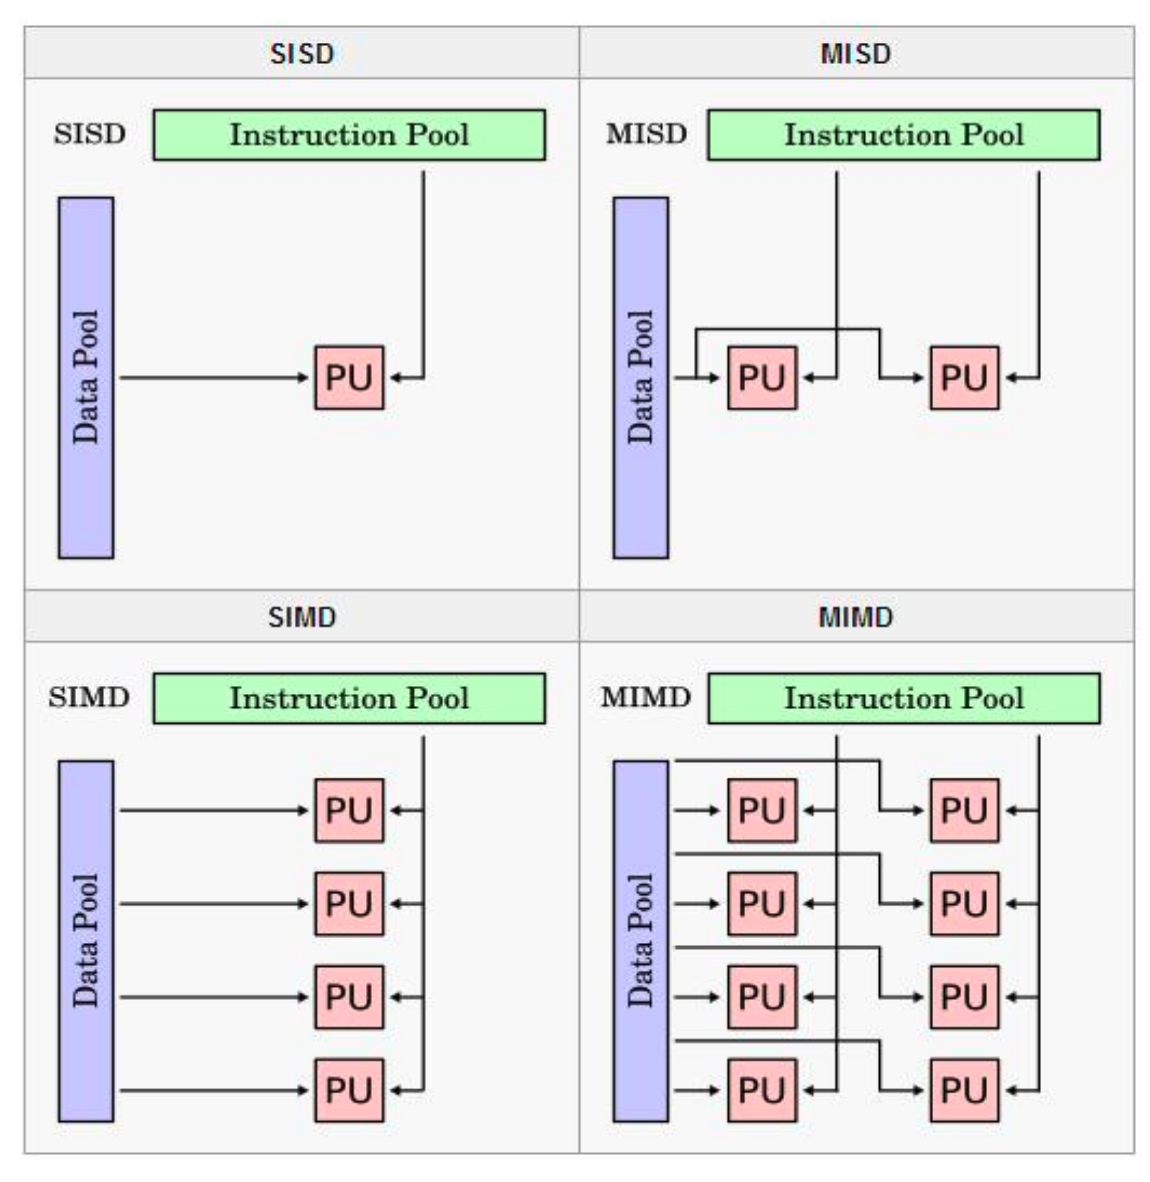
\includegraphics[width=0.7\linewidth]{figures/screenshot052}
\caption{Flynn's classifications.}
\label{fig:screenshot052}
\end{figure}


\section{Memory Architectures}
Memory architectures for a parallel computer are divided into three major categories.

\subsection{Shared Memory}
\begin{figure}
\centering
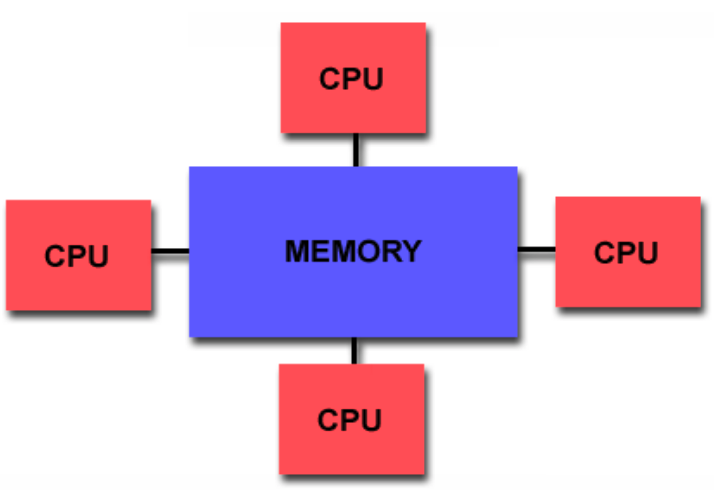
\includegraphics[width=0.5\linewidth]{figures/screenshot053}
\caption{Shared memory architecture.}
\label{fig:screenshot053}
\end{figure}

Shared memory parallel computers vary widely, but generally have in common the ability for all processors to access all memory as global address space, as seen in \autoref{fig:screenshot053}. Multiple processors can operate independently but share the same memory resources. Changes in a memory location actioned by one processor are visible to all other processors. Shared memory machines can be divided into two main classes based upon memory access times: UMA and NUMA. 

\subsection{Distributed Memory}
\begin{figure}
\centering
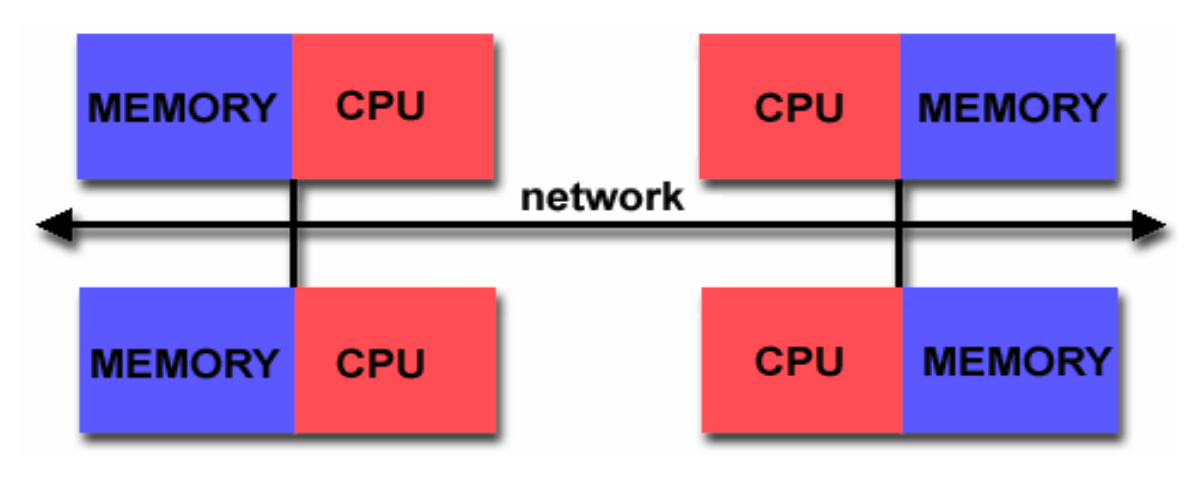
\includegraphics[width=0.5\linewidth]{figures/screenshot054}
\caption{Distributed memory architecture.}
\label{fig:screenshot054}
\end{figure}

Distributed memory systems require a communication network to connect inter-processor memory, shown in \autoref{fig:screenshot054}. Processors have their own local memory; that is, there is no global address space across all processors. As each processor has its own local memory, they operate independently - changes a processor makes to its local memory have no effect on the memory of other processors. As a result, issues with cache coherency do not generally apply \footnote{You may still have cache coherency issues if you have intra-processor parallelism (i.e. multiple cores). This is closer to a hybrid memory architecture discussed in \autoref{ssec:hybrid}.}

When a processor needs access to data in another processor, it is usually the task of the programmer to explicitly define how and when data is communicated. Synchronization between tasks is likewise the programmer's responsibility.

The network "fabric" used for data transfer varies widely, though it can be as simple as Ethernet. 

\subsection{Hybrid Memory}
\label{ssec:hybrid}
\begin{figure}
\centering
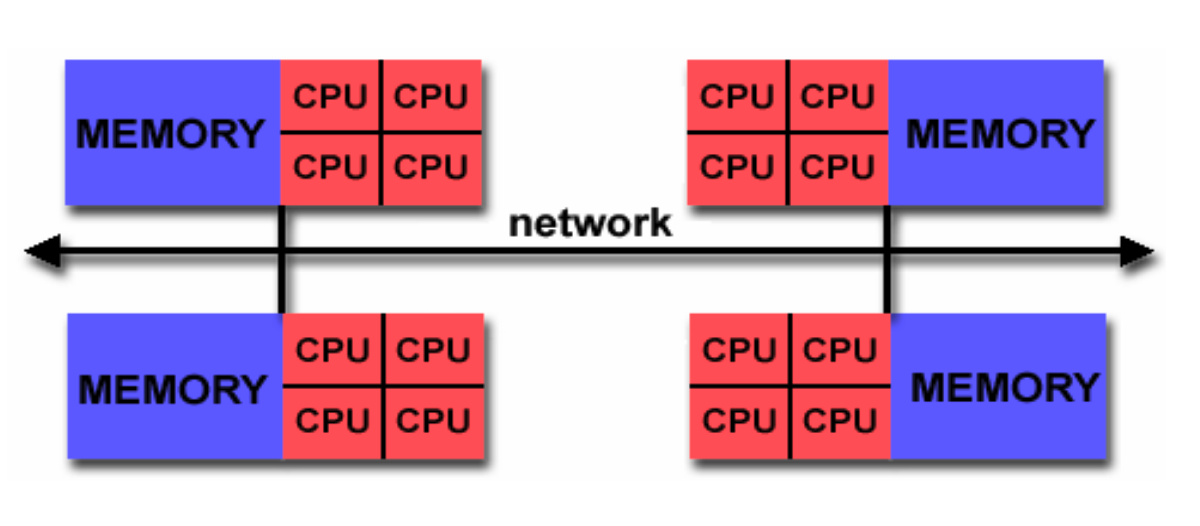
\includegraphics[width=0.5\linewidth]{figures/screenshot055}
\caption{Hybrid memory.}
\label{fig:screenshot055}
\end{figure}

The  largest and fastest computers in the world today employ both shared and distributed memory architectures. The shared memory component is usually a cache coherent SMP machine. Processors on a given SMP can address that machine's memory as global. 

The distributed memory component is the networking of multiple SMPs. SMPs know only about their own memory - not the memory on another SMP. Therefore, network communications are required to move data from one SMP to another. 

Current trends seem to indicate that this type of memory architecture will continue to prevail and increase at the high end of computing for the foreseeable future. 

The advantages and disadvantages of the hybrid model correspond to the common advantages and disadvantages of both shared and distributed memory architectures.

\section{Parallel Programming}
There are several parallel programming models in common use: \begin{itemize}
\item shared memory
\item threads
\item message passing
\item data parallelism
\item hybrid
\end{itemize}
These models exist as an abstraction above hardware and memory architectures. These models are \textit{not} specific to a particular type of machine or memory architecture; they can theoretically be implemented on any underlying hardware. This conclusion is not immediately obvious.

\subsection{Performance}
The general speed-up possible for parallel computing can be quantified using the following formula:
\[ \text{Speedup} = \frac{\text{Sequential execution time}}{\text{Parallel execution time}} \]

This can be used to determine a upper bound for parallel speedup where inherently sequential computations are $\sigma(n)$, potentially parallel computations are $\phi(n)$, and communication operations are $\kappa(n, p)$, $n$ is the problem size, and $p$ is the number of processors. Each component is investigated in \autoref{fig:screenshot056}.
\[ \psi(n,p) \le \frac{\sigma(n) + \phi(n)}{\sigma(n) + \frac{\phi(n)}{p} + \kappa(n, p)} \]

Put simply:
\[ \text{ParallelSpeedup}(n,p) \le \frac{\text{Sequential}(n) + \text{PotentiallyParallel}(n)}{\text{Sequential}(n) + \frac{\text{PotentiallyParallel}(n)}{p} + \text{Communication}(n, p)} \]

\begin{figure}
\centering
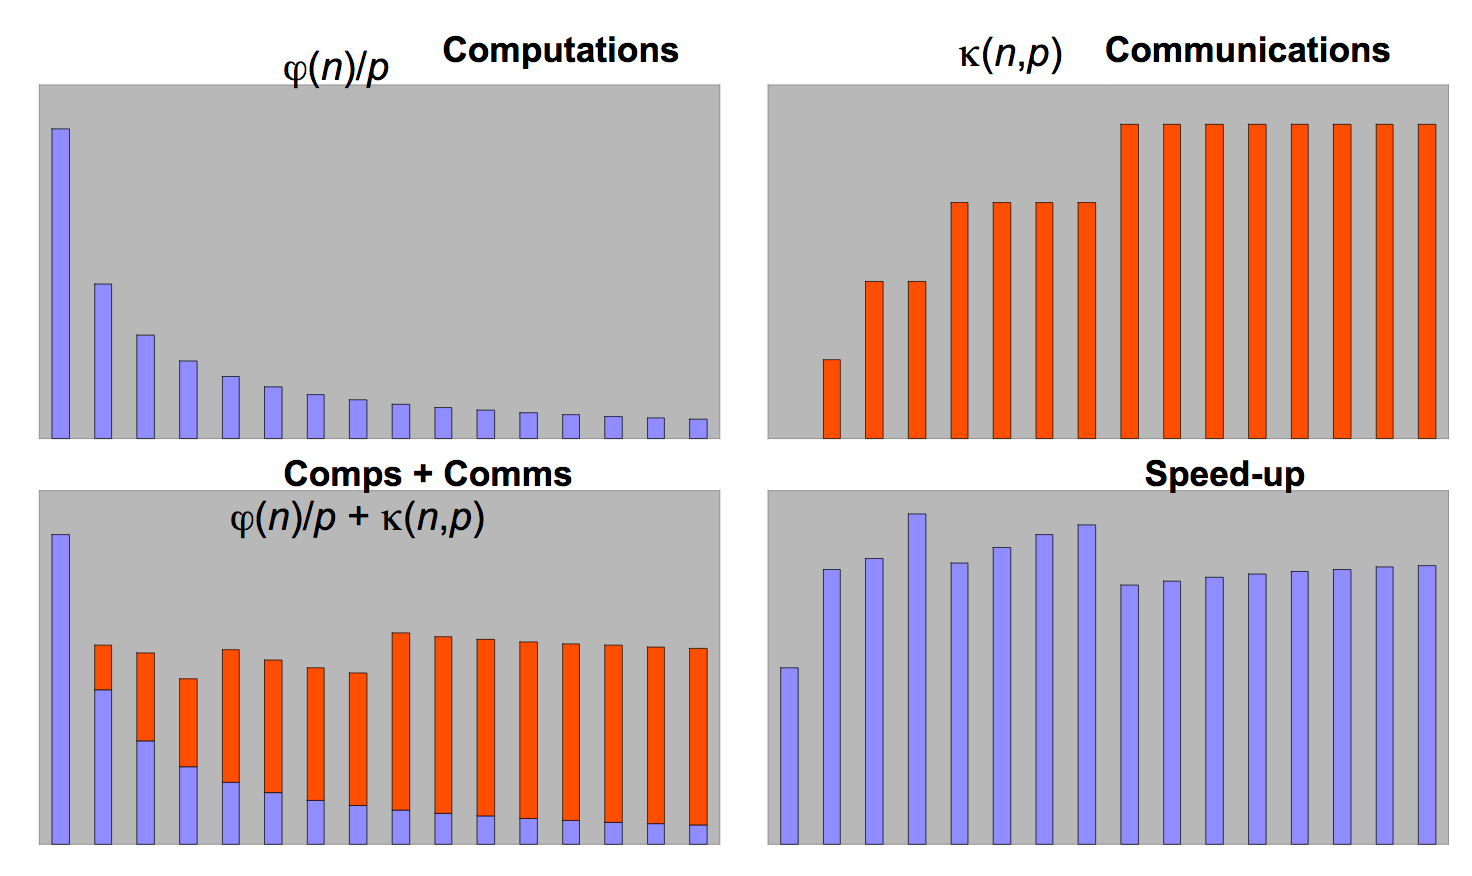
\includegraphics[width=0.7\linewidth]{figures/screenshot056}
\caption{The effect of varying values in the speed-up formula.}
\label{fig:screenshot056}
\end{figure}

\subsubsection{Amdahl's Law}
Amdahl's law states that a small portion of the program which cannot be parallelized will limit the overall speed-up available from parallelization. 

Any large mathematical or engineering problem will typically consist of several parallelizable parts and several non-parallelizable (sequential) parts. This relationship is given by the equation
\[ S = \frac{1}{1 - P} \]
where $S$ is the speedup of the program (as a factor of its original sequential runtime), and $P$ is the fraction that is parallelisable. 

\begin{figure}
\centering
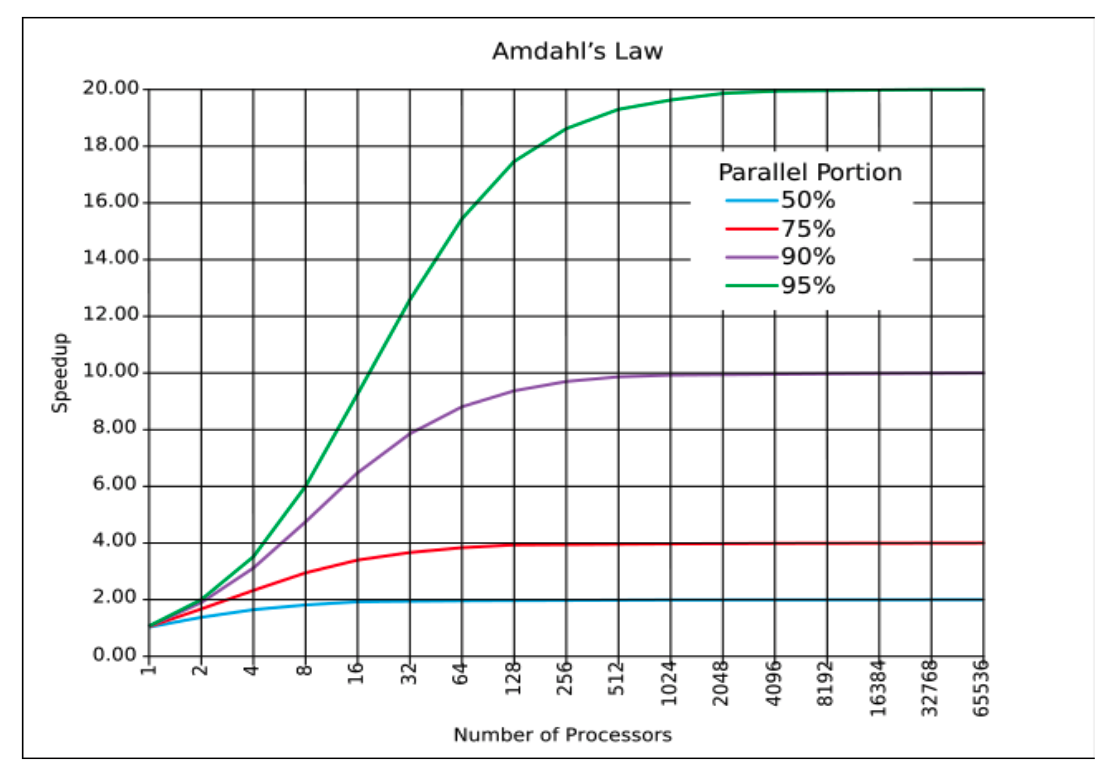
\includegraphics[width=0.7\linewidth]{figures/screenshot057}
\caption{Consequences of Amdahl's law.}
\label{fig:screenshot057}
\end{figure}

This leads to the consequence that if the sequential portion of a program is 10\% of the runtime, we can get no more than a 10x speed-up, regardless of how many processors are added. This puts an upper limit on the usefulness of adding more parallel execution units.  This is shown in \autoref{fig:screenshot057}.

Amdahl's law can be derived by altering the general speedup formula:
\[ \psi(n,p) \le \frac{\sigma(n) + \phi(n)}{\sigma(n) + \frac{\phi(n)}{p} + \kappa(n, p)} \]
Remove the communication overhead (this will result in a larger upper bound):
\[ \psi(n,p) \le \frac{\sigma(n) + \phi(n)}{\sigma(n) + \frac{\phi(n)}{p}} \]
Let $f = \frac{\sigma(n)}{\sigma(n) + \phi(n)}$; that is, $f$ is the fraction of the code which is inherently sequential. This leads to the complete formulation, which is a simplification of the general speedup formula:
\[ \psi \le \frac{1}{f + \frac{1-f}{p}} \]

Examples of using Amdahl's Law: \begin{itemize}
\item 95\% of a program’s execution time occurs inside a loop that can be executed in parallel. What is the maximum speedup we should expect from a parallel version of the program executing on 8 CPUs? 
\[ \psi \le \frac{1}{f + \frac{1-f}{p}} = \psi \le \frac{1}{0.05 + \frac{0.95}{8}} = 5.9 \]
\item 20\% of a program’s execution time is spent within inherently sequential code. What is the limit to the speedup achievable by a parallel version of the program?
\[ \lim_{p\rightarrow\infty} \frac{1}{0.2 + \frac{1-0.2}{p}} = \frac{1}{0.2} = 5 \]
\end{itemize}

Amdahl's law ignores the communication overhead, so it overestimates the possible speedup. It also assumes that $f$ is constant, which may lead to the achievable speedup being underestimated. 

The Amdahl effect refers to the potential speedup increasing with a larger $n$. This is due to the communication overhead $\kappa(n,p)$ typically having lower complexity than $\frac{\phi(n)}{p}$; as $n$ increases, $\frac{\phi(n)}{p} \gg \kappa(n,p)$, resulting in the speedup increasing and $f$ decreasing.

\subsubsection{Gustafson's Law}
Gustafson's Law (also known as Gustafson-Barsis' law, 1988) states that any sufficiently large problem can be efficiently parallelized. Gustafson's Law is closely related to Amdahl's law, which gives a limit to the degree to which a program can be sped up due to parallelization:
\[ S(P) = P-\alpha * (P - 1) \]
where $P$ is the number of processors, $S$ is the speedup, and $\alpha$ the non-parallelizable part of the process.

Gustafson's law addresses the shortcomings of Amdahl's law, which cannot scale to match availability of computing power as the machine size increases.  

It also removes the fixed problem size or fixed computation load on the parallel processors: instead, he proposes a fixed time concept which leads to scaled speed up. Amdahl's law is based on fixed workload or fixed problem size. It implies that the sequential part of a program does not change with respect to machine size (i.e, the number of processors). However, the parallel part is evenly distributed by $n$ processors. 

\subsection{Examples}
\subsubsection{Independent 2D grid}
This example demonstrates calculations on 2-dimensional array elements, with the computation on each array element being independent from other array elements (see \autoref{fig:screenshot058}).  As the calculations are independent of one another, it is an \textit{embarrassingly parallel situation}. For best use of resources, the problem should be computationally intensive.

\begin{figure}
\centering
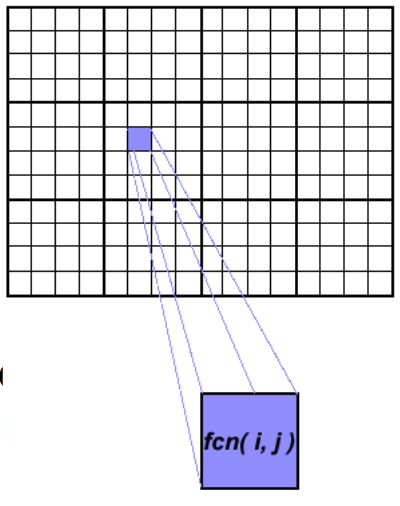
\includegraphics[width=0.3\linewidth]{figures/screenshot058}
\caption{Embarrassingly-parallel 2D grid parallel programming problem.}
\label{fig:screenshot058}
\end{figure}


The serial program calculates one element at a time in sequential order. Pseudocode for this is shown in \autoref{alg:2dserial}.
\begin{algorithm}  
\caption{Serial algorithm for computing elements in a 2D grid.}
\label{alg:2dserial}
\begin{algorithmic}
\For{j = 1, n}
	\For {i = 1, m}
		\State $\mathtt{a}(i,j) \gets \mathtt{fcn}(i,j)$
	\EndFor
\EndFor
\end{algorithmic}
\end{algorithm}

For the parallel solution, array elements are distributed so that each processor owns a portion of the array (subarray); see \autoref{fig:screenshot059}. Independent calculation of array elements ensures there is no need for communication between tasks.  Distribution scheme is chosen by other criteria, e.g. unit stride (stride of 1) through the subarrays. Unit stride maximizes cache/memory usage.
\begin{figure}
\centering
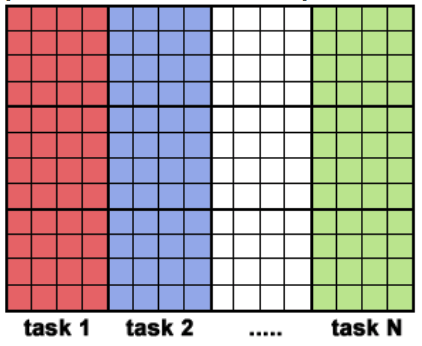
\includegraphics[width=0.4\linewidth]{figures/screenshot059}
\caption{Partitioning of the 2D grid problem for each task.}
\label{fig:screenshot059}
\end{figure}


After the array is distributed, each task executes the portion of the loop corresponding to the data it owns. This is shown in \autoref{alg:2dparallel1}.
\begin{algorithm}  
\caption{Parallel algorithm for computing elements in a 2D grid.}
\label{alg:2dparallel1}
\begin{algorithmic}
\For{j = mystart, myend}
	\For {i = 1, m}
		\State $\mathtt{a}(i,j) \gets \mathtt{fcn}(i,j)$
	\EndFor
\EndFor
\end{algorithmic}
\end{algorithm}
Note that only the outer loop variables are different from the serial solution.

Pseudocode for each node is shown in \autoref{alg:2dparallel2}.
\begin{algorithm}  
\caption{Complete parallel algorithm for computing elements in a 2D grid.}
\label{alg:2dparallel2}
\begin{algorithmic}
\If{am i the master?}
	\State initialize array
	\State send each worker info on part of array it owns  
	\State send each worker its portion of initial array  
	\State receive results from each worker
\Else
	\State receive information on which part of the array this worker owns
	\State receive the part of the array this worker owns
	\For{j = mystart, myend}
		\For {i = 1, m}
			\State $\mathtt{a}(i,j) \gets \mathtt{fcn}(i,j)$
		\EndFor
	\EndFor
	\State send results to master
\EndIf
\end{algorithmic}
\end{algorithm}

\subsubsection{Pi calculation}
\begin{figure}
\centering
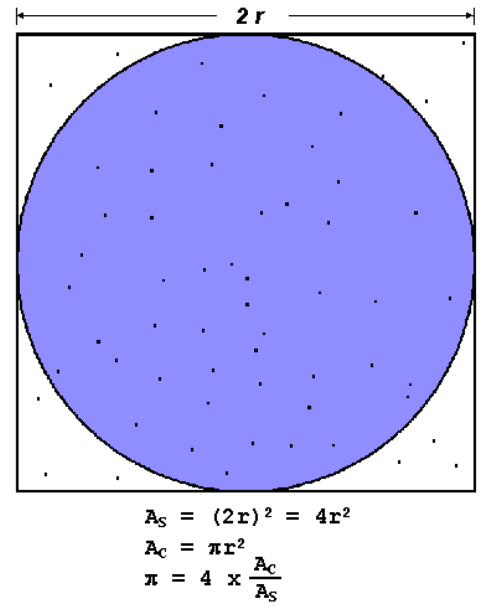
\includegraphics[width=0.4\linewidth]{figures/screenshot060}
\caption{Calculating $\pi$ through Monte Carlo sampling of a circle inside a square.}
\label{fig:screenshot060}
\end{figure}
The value of $\pi$ can be calculated through a variety of means. The algorithm chosen here is simple (depicted in \autoref{fig:screenshot060}): \begin{itemize}
\item Inscribe a circle in a square.
\item Randomly generate points in the square.
\item Determine the number of points in the square that area that are also in the circle.
\item Let $r$ be the number of points in the circle divided by the number of points in the square.
\item Finally, $\pi \approx 4r$. The approximation is improved by increasing the number of points generated.
\end{itemize}

The serial pseudocode is shown in \autoref{alg:piserial}.
\begin{algorithm}  
\caption{Serial algorithm for computing $\pi$.}
\label{alg:piserial}
\begin{algorithmic}
\State $points_{total} \gets 10000$
\State $points_{circle} \gets 0$
\For{j = 1, $points_{total}$}
	\State $(x, y) = \Call{random}{0, 1}$
	\If{\Call{inside\_circle}{x, y}}
		\State $points_{circle} \gets points_{circle} + 1$
	\EndIf
\EndFor
\State $\pi \approx 4 \times \frac{points_{circle}}{points_{total}}$
\end{algorithmic}
\end{algorithm}
From this pseudocode, it can be seen that the majority of the time spent running this program is spent in the loop, and that the algorithm itself is embarrassingly parallel. It is computationally intensive and requires little communication or I/O.

The parallel solution for this problem modifies the serial pseudocode by breaking the loop into portions that can be executed by each task. Each task can execute its portion of the loop a number of times. Each task can do its work without requiring any information from the other tasks (there are no data dependencies). This is implemented using the Single Process, Multiple Data (SPMD) model, which is a subset of MIMD; one task acts as the master and collects the results from the other processes. The pseudocode is shown in \autoref{alg:piparallel}.
\begin{algorithm}  
\caption[Parallel algorithm for computing $\pi$.]{Parallel algorithm for computing $\pi$. Each worker task calculates a number of samples that were inside the circle; these are then sent to the master, which adds them together and computes a final estimate of $\pi$.}
\label{alg:piparallel}
\begin{algorithmic}
\State $points_{total} \gets 10000$
\State $points_{circle} \gets 0$
\State $p \gets \text{number of tasks}$
\State $num \gets \frac{points_{total}}{p}$
\For{j = 1, $num$}
	\State $(x, y) = \Call{random}{0, 1}$
	\If{\Call{inside\_circle}{x, y}}
		\State $points_{circle} \gets points_{circle} + 1$
	\EndIf
\EndFor
\If{am i the master?}
	\State $points_{circle} \gets points_{circle} + \sum_p \Call{receive}{p}$
	\State $\pi \approx 4 \times \frac{points_{circle}}{points_{total}}$
\Else
	\State \Call{send}{master, $points_{circle}$}
\EndIf
\end{algorithmic}
\end{algorithm}

\subsubsection{1-D Wave Equation}
\begin{figure}
\centering
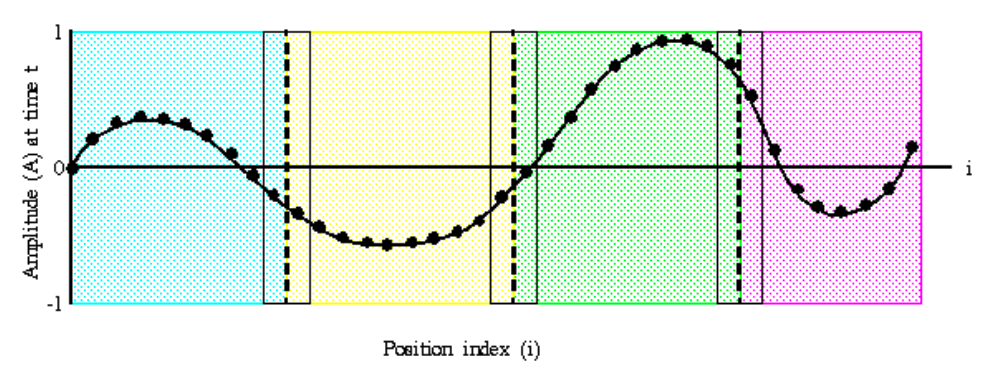
\includegraphics[width=0.7\linewidth]{figures/screenshot061}
\caption{Parallel 1-D wave equation.}
\label{fig:screenshot061}
\end{figure}

Implemented with the SPMD model. The entire amplitude array is partitioned and distributed as sub-arrays to all tasks, as seen in \autoref{fig:screenshot061}. Each task owns a portion of the total array. All points require equal work, so the points should be divided equally. A block decomposition would have the work partitioned into the number of tasks as chunks, allowing each task to own mostly contiguous data points. 

Communication only needs to occur on data borders. The larger the block size, the less the communication. The equation to be solved is the one-dimensional wave equation:  
\[ A(i, t+1) = (2.0 \times A(i, t)) - A(i, t-1) + (c \times (A(i-1, t) - (2.0 \times A(i, t)) + A(i+1, t))) \]
where $c$ is a constant.

\begin{algorithm}[h]
\caption{Parallel algorithm for computing the 1-D wave equation. \footnotemark}
\label{alg:screenshot062}
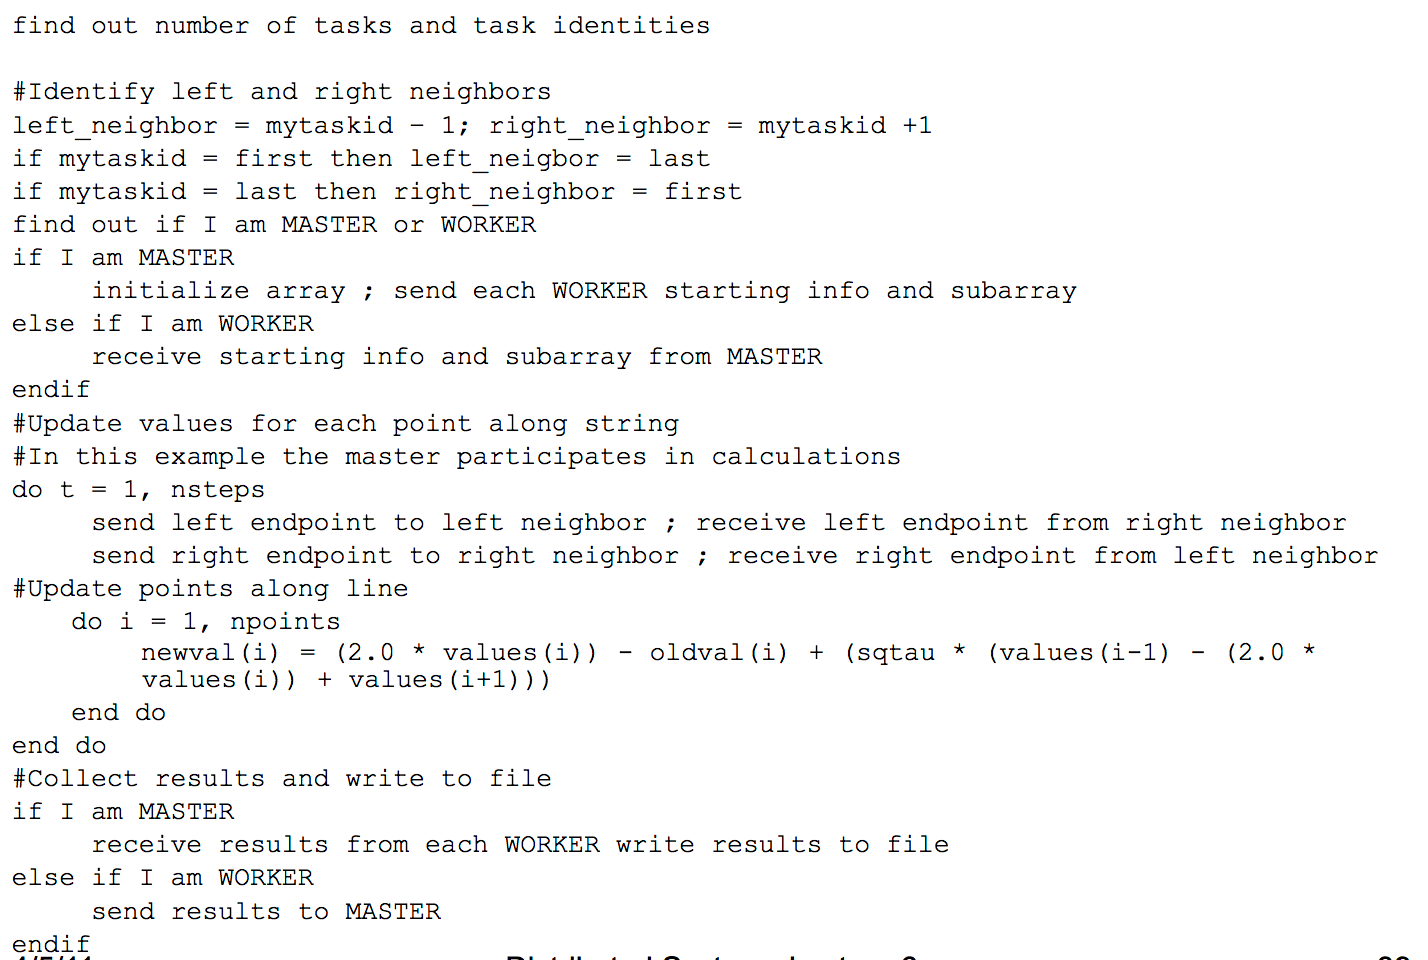
\includegraphics[width=\linewidth]{figures/screenshot062}
\end{algorithm}
\footnotetext{I didn't want to transcribe this to pseudocode properly. Sorry!}

Note that the amplitude will depend on previous timesteps $(t, t-1)$ and neighboring points $(i-1, i+1)$. This data dependence will mean that a parallel solution will require communication. This parallel solution is depicted in \autoref{alg:screenshot062}.
